% ============================================================
%  SECTION 3 — PROBLEM FORMULATION
% ============================================================

This section develops the complete mathematical formulation of the
portfolio budget allocation problem and its specification as a
Gymnasium-compatible reinforcement learning environment. The section
is structured as follows. Section~\ref{subsec:problem_statement}
states the problem scope and structural assumptions.
Section~\ref{subsec:environment} defines the environment primitives:
project dynamics, FIDIC contract cash-flow mechanics, EVM performance
signals, the termination mechanic, and portfolio balance.
Section~\ref{subsec:parameters} consolidates all parameters.
Section~\ref{subsec:theoretical_ub} establishes the deterministic
full-foresight upper bound and the information-theoretic argument for
why the stochastic problem cannot be solved by enumeration.
Section~\ref{subsec:mdp} formulates the problem as a Markov Decision
Process (MDP), defining the state space, action space, transition
kernel, and reward function that constitute the environment's
mathematical contract.

% ------------------------------------------------------------
\subsection{Problem Statement and Scope}
\label{subsec:problem_statement}
% ------------------------------------------------------------

A portfolio of $n$contracted projects is fixed: commitments are signed, start dates are
scheduled, and contracts are parameterised consistently with FIDIC Red,
Yellow, and Silver Book forms \citep{FIDIC2017}. The decision-maker ---
a portfolio manager, board, or programme director --- exercises a single
recurring lever at each discrete planning period $t \in \mathcal{T} =
\{0, 1,\ldots,H-1\}$: the budget $x_{i,t} \geq 0$ directed to each
active project $i$. The planning horizon $H$ is determined endogenously
as $H = \max_i (f_i + \Delta^{\max}_i)$, where $f_i$ is the planned
finish of project $i$ and $\Delta^{\max}_i$ is the maximum permitted
overrun; period $t = 0$ aligns with the earliest project start. All
outcomes of interest --- milestone achievement, cash inflows, schedule
adherence, and project termination --- flow through this allocation
decision. Portfolio selection is treated as an exogenous upstream input
\citep{Archer1999}.

Four structural assumptions underlie the formulation.

\begin{enumerate}[label=(\roman*)]
  \item \emph{Independent bilateral contracts.} Projects interact
    only through the shared cash balance; no resource or workforce
    sharing occurs, consistent with standard EPC contracting practice.

  \item \emph{Budget as the sole control.} The contractor's internal
    resource decisions are absorbed into a stochastic efficiency
    parameter $\eta_{i,t}$; the portfolio manager observes how much
    physical progress a budget allocation yields, not how it is
    achieved. $\eta_{i,t}$ is the sole stochastic primitive: it is
    unobservable at the time allocation $x_{i,t}$ is committed, and
    its realisation determines whether and when each milestone
    threshold is crossed.

  \item \emph{Discrete monthly periods.} $\mathcal{T} =
    \{0,\ldots,H-1\}$ reflects the standard monthly governance cycle
    of portfolio management. A configurable budget tightness ratio
    $\kappa = B_0 / \sum_i \mathrm{BAC}_i$ parameterises the liquidity
    regime across configurations.

  \item \emph{FIDIC contract mechanics.} Milestone payments, advance
    payment and recovery, retention, and termination settlement are
    all configurable parameters, accommodating the full range of
    particular conditions encountered in practice.
\end{enumerate}

% ------------------------------------------------------------
\subsection{Environment Definition}
\label{subsec:environment}
% ------------------------------------------------------------

\begin{figure}[htbp]
  \centering
  \resizebox{\textwidth}{!}{%
  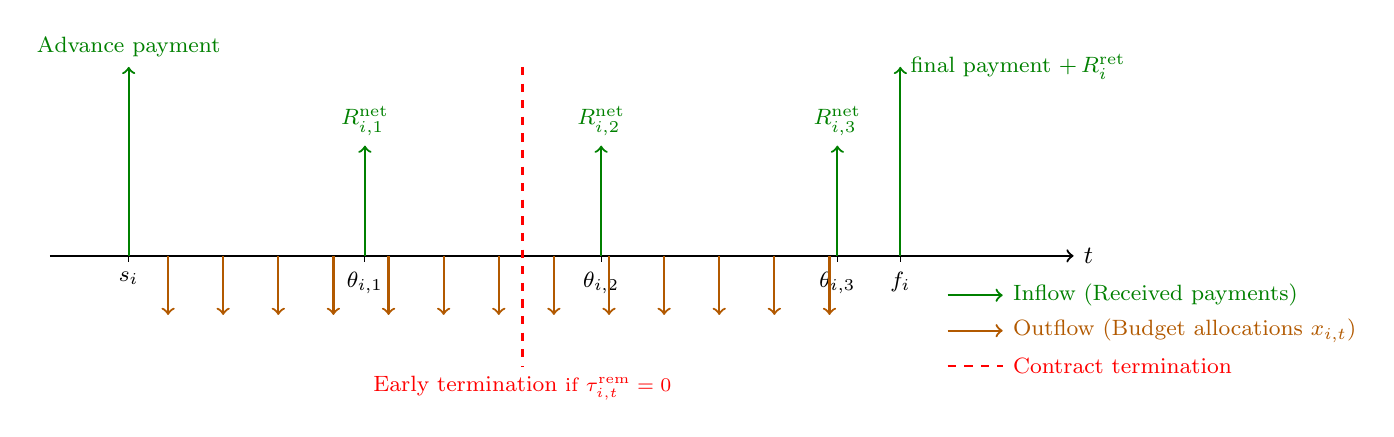
\begin{tikzpicture}[
      every node/.style={font=\small},
      inflow/.style={->, thick, green!50!black},
      outflow/.style={->, thick, orange!70!black},
      legend/.style={font=\footnotesize, align=left}
      ]

      \draw[->, thick] (0,0) -- (13.0,0) node[right] {$t$};

      \foreach \x/\lbl in {1/$s_i$, 4/$\theta_{i,1}$, 7/$\theta_{i,2}$,
                          10/$\theta_{i,3}$, 10.8/$f_i$}{
      \draw (\x,0.08) -- (\x,-0.08)
          node[below, font=\footnotesize] {\lbl};
      }

      % Contract payments
      \draw[inflow] (1,0) -- (1,2.4)
      node[above, align=center, font=\footnotesize]
          {Advance payment};

      \draw[inflow] (4,0) -- (4,1.4)
      node[above, font=\footnotesize] {$R_{i,1}^{\mathrm{net}}$};

      \draw[inflow] (7,0) -- (7,1.4)
      node[above, font=\footnotesize] {$R_{i,2}^{\mathrm{net}}$};

      \draw[inflow] (10,0) -- (10,1.4)
      node[above, align=center, font=\footnotesize]
          {$R_{i,3}^{\mathrm{net}}$};

      \draw[inflow] (10.8,0) -- (10.8,2.4)
      node[right, align=center, font=\footnotesize]
          {final payment $+\,R_i^{\mathrm{ret}}$};

      % Budget allocations (outflows)
      \foreach \x in {1.5,2.2,2.9,3.6,4.3,5.0,5.7,6.4,
                      7.1,7.8,8.5,9.2,9.9}{
      \draw[outflow] (\x,0) -- (\x,-0.75);
      }

      % Early termination
      \draw[dashed, thick, red] (6.0,2.4) -- (6.0,-1.4)
      node[below, align=center, font=\footnotesize, red]
          {Early termination {\scriptsize if $\tau_{i,t}^{\mathrm{rem}}=0$}};

      \begin{scope}[shift={(11.4,-0.5)}]
        \draw[inflow] (0,0) -- (0.7,0)
        node[right, legend] {Inflow (Received payments)};
        \draw[outflow] (0,-0.45) -- (0.7,-0.45)
        node[right, legend] {Outflow (Budget allocations $x_{i,t}$)};
        \draw[dashed, thick, red] (0,-0.9) -- (0.7,-0.9)
        node[right, legend] {Contract termination};
      \end{scope}

  \end{tikzpicture}
  }
  \caption{Cash-flow timeline for project $i$ under FIDIC contract mechanics.}
  \label{fig:cashflow_timeline}
\end{figure}


% - - - - - - - - - - - - - - - - - - - - - - - - - - - - - -
\subsubsection{Sets, Indices, and the Decision Variable}
\label{subsubsec:sets}
% - - - - - - - - - - - - - - - - - - - - - - - - - - - - - -

\begin{description}[leftmargin=2.6cm, labelwidth=2.4cm]
  \item[$\mathcal{P}$]
    Projects $\{0,\ldots,n-1\}$, indexed by $i$; all committed at
    horizon start.
  \item[$\mathcal{T}$]
    Planning periods $\{0,\ldots,H-1\}$, indexed by $t$ (calendar
    months), where $H = \max_{i \in \mathcal{P}}(f_i +
    \Delta^{\max}_i)$ is derived endogenously from the committed
    portfolio; period $t=0$ aligns with the earliest project start.
  \item[$\mathcal{M}_i$]
    Ordered milestones $\{1,\ldots,M_i\}$ for project $i$, indexed
    by $j$, with progress thresholds
    $\theta_{i,1} < \cdots < \theta_{i,M_i} = 1$.
    A synthetic milestone $j=0$ records the advance payment at
    project start $s_i$ with progress threshold zero.
  \item[$\mathcal{P}_t^{\mathrm{active}}$]
    Projects with \texttt{active} status at period $t$; endogenous to
    the efficiency trajectory and termination events.
  \item[$x_{i,t} \geq 0$]
    \textbf{Decision variable}: budget allocated to project $i$ at
    period $t$. The period-$t$ action vector is
    $\mathbf{x}_t = (x_{i,t})_{i \in \mathcal{P}_t^{\mathrm{active}}}$.
  \item[$B_t \geq 0$]
    Portfolio cash balance at the start of period $t$; $B_0$ is given.
\end{description}

% - - - - - - - - - - - - - - - - - - - - - - - - - - - - - -
\subsubsection{Progress and Expenditure Dynamics}
\label{subsubsec:progress}
% - - - - - - - - - - - - - - - - - - - - - - - - - - - - - -

Budget $x_{i,t}$ converts to physical progress through the efficiency
scalar $\eta_{i,t}$, which absorbs all sources of conversion
uncertainty (contractor productivity, supply chain, weather):
\begin{equation}
  P_{i,t}^{\mathrm{actual}}
    = \min\!\left(1,\;
        P_{i,t-1}^{\mathrm{actual}}
        + \eta_{i,t} \cdot \frac{x_{i,t}}{\mathrm{BAC}_i}
      \right),
  \qquad
  \mathrm{ACWP}_{i,t} = \mathrm{ACWP}_{i,t-1} + x_{i,t},
  \label{eq:progress_rec}
\end{equation}
with $P_{i,0}^{\mathrm{actual}} = \mathrm{ACWP}_{i,0} = 0$. Here
$\mathrm{BAC}_i$ is the Budget at Completion --- the total planned
contractor expenditure for project $i$, which serves as the EVM cost
basis and the normalisation denominator for all progress calculations.
The efficiency $\eta_{i,t}$ is realised from a project-specific
distribution only after allocation $x_{i,t}$ is committed; it is the
sole stochastic primitive. A global floor of $\eta_{i,t} \geq 0.01$
prevents degenerate zero-progress episodes.

The planned cumulative progress follows a normalised S-curve
\citep{Kenley2009, barraza2004probabilistic} parameterised by Beta
shape parameters $(a_i, b_i)$. Defining the normalised project-time
fraction $\tau_{i,t} = (t - s_i) / D_i^{\mathrm{plan}}$ clipped to
$[0,1]$, the planned progress at period $t$ is:
\begin{equation}
  P_{i,t}^{\mathrm{plan}}
    = I_{\tau_{i,t}}(a_i, b_i),
  \label{eq:scurve}
\end{equation}
where $I_\tau(\cdot,\cdot)$ is the regularised incomplete Beta function
and $D_i^{\mathrm{plan}} = f_i - s_i$ is the planned duration.
This profile is a fixed parameter derived at commitment; it is never
a decision variable.

% - - - - - - - - - - - - - - - - - - - - - - - - - - - - - -
\subsubsection{Contractual Cash-Flow Mechanics}
\label{subsubsec:cashflow}
% - - - - - - - - - - - - - - - - - - - - - - - - - - - - - -

Payment inflows follow FIDIC mechanics \citep{FIDIC2017}.
At project initiation ($t = s_i$), the portfolio manager receives an
advance payment:
\begin{equation}
  A_i = \alpha_i \cdot CP_i,
  \label{eq:advance}
\end{equation}
where $\alpha_i$ is the advance ratio and $CP_i = \mathrm{BAC}_i
(1 + \pi_i)$ is the contract price with profit margin $\pi_i$.
The contract price is the sole payment accumulation baseline: all
milestone revenues, advance payment, retention, and final settlement
sum to $CP_i$. All EVM performance signals and progress calculations
are normalised against $\mathrm{BAC}_i$.

Milestone $j \geq 1$ is certified at the first period $t$ at which
both $P_{i,t}^{\mathrm{actual}} \geq \theta_{i,j}$ and $t \geq
e_{i,j}$, where $e_{i,j} = s_i + \tau_{i,j}^{\mathrm{thresh}}$ is
the contractual earliest certification period and
$\tau_{i,j}^{\mathrm{thresh}}$ is the project-time threshold
\citep{FIDIC2017}. Certification is monotone: once certified, a
milestone remains certified. The net payment received upon
certification of milestone $j$, after retention withholding at rate
$\rho_i$ and advance recovery deduction at rate $\delta_i^{\mathrm{rec}}$
once cumulative certified payments exceed threshold $\psi_i$, is:
\begin{equation}
  R_{i,j}^{\mathrm{net}}
    = \phi_{i,j} \cdot CP_i
      - \rho_i \cdot \phi_{i,j} \cdot CP_i
      - \delta_i^{\mathrm{rec}} \cdot \phi_{i,j} \cdot CP_i
        \cdot \mathbf{1}\!\left\{
          \textstyle\sum_{k \leq j} \phi_{i,k} \geq \psi_i
        \right\}
      + \rho_i \cdot CP_i \cdot \mathbf{1}\{j = M_i\},
  \label{eq:Rnet}
\end{equation}
where $\phi_{i,j}$ is the contractual weight of milestone $j$ with
$\sum_j \phi_{i,j} = 1$. The final term releases accumulated retention
$R_i^{\mathrm{ret}} = \rho_i \cdot CP_i$ at project completion. The
payment identity $A_i + \sum_j R_{i,j}^{\mathrm{net}} = CP_i$ holds
exactly. Milestone payments are received in the same period they are
certified. The aggregate period inflow is:
\begin{equation}
  V_t
    = \sum_{i \in \mathcal{P}} \sum_{j \in \mathcal{M}_i}
        R_{i,j}^{\mathrm{net}}
        \cdot \mathbf{1}\!\left\{
          \tau_{i,j}^{\mathrm{cert}} = t
        \right\}
      + \sum_{i \in \mathcal{P}_t^{\mathrm{term}}} R_i^{\mathrm{term}},
  \label{eq:Vt}
\end{equation}
where $\mathcal{P}_t^{\mathrm{term}}$ collects projects newly
terminated at $t$ and $R_i^{\mathrm{term}}$ is defined in
Section~\ref{subsubsec:termination}.

% - - - - - - - - - - - - - - - - - - - - - - - - - - - - - -
\subsubsection{Performance Monitoring: EVM Signals}
\label{subsubsec:evm}
% - - - - - - - - - - - - - - - - - - - - - - - - - - - - - -

The Earned Value Management framework \citep{Fleming2010} provides the
diagnostic vocabulary used to monitor contractor performance and to
drive the termination mechanic. The Earned Value at period $t$ is
$\mathrm{EV}_{i,t} = P_{i,t}^{\mathrm{actual}} \cdot \mathrm{BAC}_i$.
The project-time elapsed since project start is denoted
$\tau_i^{\mathrm{proj}}(t) = t - s_i$. Four derived indices are
computed each period.

The Schedule Performance Index uses the Earned Schedule formulation
\citep{Lipke2003}. The Earned Schedule $\mathrm{ES}_{i,t}$ is the
value $\tau^* \in [0, D_i^{\mathrm{plan}}]$ satisfying
$I_{\tau^*/D_i^{\mathrm{plan}}}(a_i, b_i) = P_{i,t}^{\mathrm{actual}}$,
computed by binary search over the Beta CDF:
\begin{align}
  \mathrm{SPI}_{i,t}
    &= \frac{\mathrm{ES}_{i,t}}{\tau_i^{\mathrm{proj}}(t)},
  \label{eq:SPI} \\
  \mathrm{CPI}_{i,t}
    &= \frac{\mathrm{EV}_{i,t}}{\mathrm{ACWP}_{i,t}},
  \label{eq:CPI} \\
  \mathrm{EAC}_{i,t}
    &= \mathrm{ACWP}_{i,t}
       + \frac{\mathrm{BAC}_i - \mathrm{EV}_{i,t}}
              {\mathrm{CPI}_{i,t} \cdot \mathrm{SPI}_{i,t}},
  \label{eq:EAC} \\
  \mathrm{TCPI}_{i,t}
    &= \frac{\mathrm{BAC}_i - \mathrm{EV}_{i,t}}
            {\mathrm{BAC}_i - \mathrm{ACWP}_{i,t}}.
  \label{eq:TCPI}
\end{align}

Unlike the classical $\mathrm{SPI} = \mathrm{EV}/\mathrm{PV}$, which
freezes once the planned value reaches $\mathrm{BAC}_i$ at planned
finish, the Earned Schedule formulation \eqref{eq:SPI} degrades
continuously as real time passes without progress, correctly
distinguishing a project one period late from one three periods late
\citep{Lipke2003}. This formulation is adopted throughout. The
composite denominator $\mathrm{CPI}_{i,t} \cdot \mathrm{SPI}_{i,t}$
in \eqref{eq:EAC} incorporates both cost and schedule underperformance
into the cost-at-completion forecast. $\mathrm{TCPI}_{i,t}$ measures
the cost efficiency that must be sustained on remaining work to finish
within $\mathrm{BAC}_i$; values above 1.10 are widely considered
unrecoverable \citep{Fleming2010, christensen1993est}. All four indices
are observable state components. Denominators that would produce
undefined results default to one (no overrun implied), consistent with
the project state before any expenditure has been committed.

% - - - - - - - - - - - - - - - - - - - - - - - - - - - - - -
\subsubsection{Termination Mechanic}
\label{subsubsec:termination}
% - - - - - - - - - - - - - - - - - - - - - - - - - - - - - -

Termination is an endogenous environment mechanic, not an agent action.
Two conditions are evaluated for every active project at each period.

\paragraph{Condition 1 — Progress delay breach.}
The progress lag at period $t$ is:
\begin{equation}
  \delta_{i,t} = P_{i,t}^{\mathrm{plan}} - P_{i,t}^{\mathrm{actual}}.
  \label{eq:progress_lag}
\end{equation}
Condition~1 activates when this lag exceeds the contractual cap:
\begin{equation}
  \delta_{i,t} > \delta^{\max}_i,
  \label{eq:term_cond1}
\end{equation}
where $\delta^{\max}_i \in [0,1]$ is the project-specific tolerance
fixed at commitment, grounded in the FIDIC engineer's authority to
issue a notice when progress falls materially behind programme
\citep{FIDIC2017}.

\paragraph{Condition 2 — Hard deadline breach.}
A hard deadline fires unconditionally at:
\begin{equation}
  t \geq f_i + \Delta^{\max}_i,
  \label{eq:term_cond2}
\end{equation}
where $\Delta^{\max}_i \in \mathbb{Z}^+$ is the maximum permitted
finish overrun in periods. This triggers immediate termination
regardless of the cure-period counter state.

\paragraph{Cure-period counter and termination execution.}
When Condition~1 is active the environment decrements a project-specific
cure-period counter, modelling the FIDIC Sub-Clause~15.1 obligation
to allow a recovery interval before termination may be executed
\citep{FIDIC2017, Ndekugri2008}:
\begin{equation}
  \tau^{\mathrm{rem}}_{i,t}
    = \begin{cases}
        \max\!\left(0,\; \tau^{\mathrm{rem}}_{i,t-1} - 1\right)
          & \text{if \eqref{eq:term_cond1} holds,} \\
        \tau_i^{\mathrm{tol}}
          & \text{if \eqref{eq:term_cond1} lapses.}
      \end{cases}
  \label{eq:counter}
\end{equation}
The counter initialises at $\tau^{\mathrm{rem}}_{i,s_i} =
\tau_i^{\mathrm{tol}}$, where $\tau_i^{\mathrm{tol}} \in \mathbb{Z}^+$
is fixed at commitment. Soft termination executes when the counter
reaches zero: $t_i^{\mathrm{term}} = \min\{t :
\tau^{\mathrm{rem}}_{i,t} = 0\}$. Hard termination
\eqref{eq:term_cond2} overrides the counter and executes immediately.
Condition~2 is evaluated in the early phase of each period (before
allocation); Condition~1 and counter updates apply in the late phase
(after allocation and progress realisation). The counter is part of
the observable state; the agent influences it indirectly through
allocations that drive $P_{i,t}^{\mathrm{actual}}$ relative to
$P_{i,t}^{\mathrm{plan}}$.

Upon termination at $t_i^{\mathrm{term}}$, the net settlement is:
\begin{equation}
  R_i^{\mathrm{term}}
    = P_{i,t_i^{\mathrm{term}}}^{\mathrm{actual}} \cdot CP_i
      - \mathrm{cumInflow}_{i,t_i^{\mathrm{term}}},
  \label{eq:term_settlement}
\end{equation}
where $\mathrm{cumInflow}_{i,t}$ is the cumulative inflow received
for project $i$ through period $t$ (advance payment plus all net
milestone payments certified up to and including $t$). The first term
is the contractor's entitlement for work physically delivered; the
second is what has already been collected. Positive
$R_i^{\mathrm{term}}$ arises when delivered work exceeds cumulative
receipts; negative $R_i^{\mathrm{term}}$ constitutes a net contractor
obligation (large advance not yet recovered by certified milestones).
In either case the settlement is fully determined by contract
parameters and the progress level at termination.

\begin{figure}[htbp]
  \centering
  \resizebox{\textwidth}{!}{%
  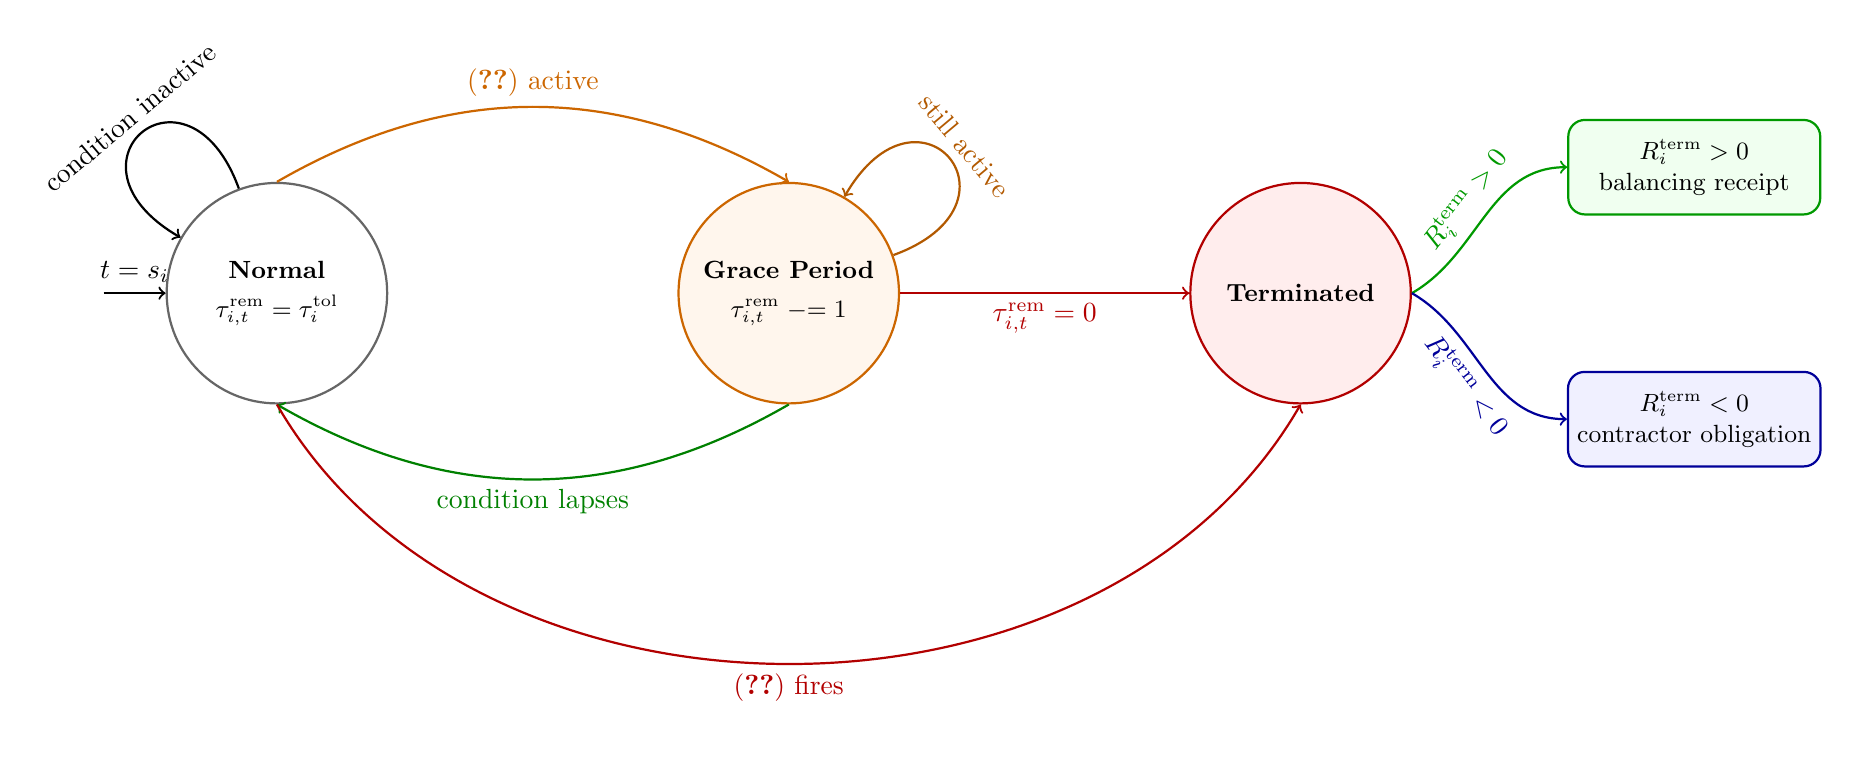
\begin{tikzpicture}[
      every node/.style={font=\small},
      state/.style={circle, draw=black!60, fill=white,
                    minimum size=2.8cm, align=center, thick},
      grace/.style={circle, draw=orange!80!black, fill=orange!7,
                    minimum size=2.8cm, align=center, thick},
      term/.style={circle, draw=red!70!black, fill=red!7,
                    minimum size=2.8cm, align=center, thick},
      posnode/.style={rectangle, rounded corners=6pt,
                  draw=green!60!black, fill=green!6,
                  minimum width=3.2cm, minimum height=1.2cm,
                  align=center, thick},
      negnode/.style={rectangle, rounded corners=6pt,
                  draw=blue!60!black, fill=blue!6,
                  minimum width=3.2cm, minimum height=1.2cm,
                  align=center, thick},
    ]

    \node[state] (normal) at (0,0)
      {\textbf{Normal}\\[3pt]
        $\tau_{i,t}^{\mathrm{rem}} = \tau_i^{\mathrm{tol}}$};

    \node[grace] (grace) at (6.5,0)
      {\textbf{Grace Period}\\[3pt]
        $\tau_{i,t}^{\mathrm{rem}} \mathrel{-}= 1$};

    \node[term] (term) at (13,0)
      {\textbf{Terminated}};

    \node[posnode] (posout) at (18,1.6)
      {$R_i^{\mathrm{term}} > 0$\\balancing receipt};

    \node[negnode] (negout) at (18,-1.6)
      {$R_i^{\mathrm{term}} < 0$\\contractor obligation};

    \draw[->, thick] (-2.2,0) -- (normal.west)
      node[midway, above, font=\normalsize] {$t = s_i$};

    \draw[->, thick, orange!80!black]
      (normal.north) to[out=30, in=150]
      node[above, font=\normalsize, align=center]
        {(\ref{eq:term_cond1}) active}
      (grace.north);

    \draw[->, thick, green!50!black]
      (grace.south) to[out=210, in=330]
      node[below, font=\normalsize, align=center]
        {condition lapses}
      (normal.south);

    \draw[->, thick, orange!70!black]
      (grace) to[out=20, in=60, looseness=5]
      node[above, font=\normalsize, sloped]
        {still active}
      (grace);

    \draw[->, thick, red!70!black] (grace.east) -- (term.west)
      node[midway, below, font=\normalsize, align=center]
        {$\tau_{i,t}^{\mathrm{rem}} = 0$};

    \draw[->, thick, black]
      (normal) to[out=110, in=150, looseness=5]
      node[above, font=\normalsize, sloped] {condition inactive}
      (normal);

    \draw[->, thick, red!70!black]
      (normal.south) to[out=-60, in=-120]
      node[below, font=\normalsize, align=center]
        {(\ref{eq:term_cond2}) fires}
      (term.south);

    \draw[->, thick, green!60!black]
      (term.east) to[out=30, in=180]
      node[midway, above, font=\normalsize, sloped]
        {$R_i^{\mathrm{term}} > 0$}
      (posout.west);

    \draw[->, thick, blue!60!black]
      (term.east) to[out=-30, in=180]
      node[midway, below, font=\normalsize, sloped]
        {$R_i^{\mathrm{term}} < 0$}
      (negout.west);

  \end{tikzpicture}%
  }
  \caption{Finite-state representation of the termination mechanic for
    project $i$.}
  \label{fig:state_machine}
\end{figure}

% - - - - - - - - - - - - - - - - - - - - - - - - - - - - - -
\subsubsection{Portfolio Cash Balance}
\label{subsubsec:balance}
% - - - - - - - - - - - - - - - - - - - - - - - - - - - - - -

The portfolio cash balance evolves as:
\begin{equation}
  B_{t+1}
    = B_t
      - \sum_{i \in \mathcal{P}_t^{\mathrm{active}}} x_{i,t}
      + V_t.
  \label{eq:balance}
\end{equation}
The shared balance $B_t$ is the sole coupling across otherwise
independent project dynamics. The budget tightness ratio
$\kappa = B_0 / \sum_i \mathrm{BAC}_i$ parameterises the liquidity
regime: $\kappa \gg 1$ (relaxed, liquidity non-binding),
$\kappa \approx 1$ (tight), $\kappa \ll 1$ (scarce). When
$B_t \leq 0$ and no advance payments are pending, the episode
truncates immediately as no further progress is achievable.

% ------------------------------------------------------------
\subsection{Consolidated Parameter Reference}
\label{subsec:parameters}
% ------------------------------------------------------------

Table~\ref{tab:params} lists all parameters fixed at commitment,
grouped by function.

\begin{table}[htbp]
  \centering\small
  \renewcommand{\arraystretch}{1.3}
  \setlength{\tabcolsep}{6pt}
  \begin{tabular}{>{\bfseries}p{3.2cm} p{1.9cm} p{1.2cm} p{7.2cm}}
    \toprule
    \normalfont\textbf{Parameter} & \textbf{Symbol} &
    \textbf{Domain} & \textbf{Definition} \\
    \midrule
    \multicolumn{4}{l}{\textit{Schedule}} \\
    \midrule
    \rowcolor{RowAlt}
    Planned start \& finish
      & $s_i,\;f_i$ & $\mathbb{Z}^+_0$
      & Anchor of execution window and S-curve. \\
    Planned duration
      & $D_i^{\mathrm{plan}}$ & $\mathbb{Z}^+$
      & $f_i - s_i$; normalises project-time for S-curve. \\
    \rowcolor{RowAlt}
    S-curve shape
      & $a_i,\;b_i$ & $\mathbb{R}^+$
      & Beta CDF parameters governing planned expenditure
        profile \eqref{eq:scurve}. \\
    Milestone progress threshold
      & $\theta_{i,j}$ & $(0,1]$
      & Cumulative progress fraction required to certify
        milestone $j$; $\theta_{i,M_i} = 1$. \\
    \rowcolor{RowAlt}
    Milestone timestep threshold
      & $\tau_{i,j}^{\mathrm{thresh}}$ & $\mathbb{Z}^+_0$
      & Project-time period at which milestone $j$ becomes
        eligible for certification; enforces FIDIC Sub-Clause~14.3
        payment interval constraints \citep{FIDIC2017}. \\
    Progress delay cap
      & $\delta^{\max}_i$ & $[0,1]$
      & Maximum admissible progress lag before Condition~1
        \eqref{eq:term_cond1} activates. \\
    \rowcolor{RowAlt}
    Finish delay cap
      & $\Delta^{\max}_i$ & $\mathbb{Z}^+$
      & Maximum permitted finish overrun in periods before
        hard deadline \eqref{eq:term_cond2} fires. \\
    Termination tolerance
      & $\tau_i^{\mathrm{tol}}$ & $\mathbb{Z}^+$
      & Cure-period length; models FIDIC Sub-Clause~15.1
        \citep{FIDIC2017, Ndekugri2008}. \\
    \midrule
    \multicolumn{4}{l}{\textit{Contract}} \\
    \midrule
    \rowcolor{RowAlt}
    Contract price
      & $CP_i$ & $\mathbb{R}^+$
      & Total client payment; $CP_i = \mathrm{BAC}_i(1+\pi_i)$. \\
    Budget at completion
      & $\mathrm{BAC}_i$ & $\mathbb{R}^+$
      & Total planned contractor expenditure; EVM cost basis and
        progress normalisation denominator. \\
    \rowcolor{RowAlt}
    Profit margin
      & $\pi_i$ & $\mathbb{R}^+_0$
      & Contractual markup on $\mathrm{BAC}_i$. \\
    Advance payment ratio
      & $\alpha_i$ & $[0,1]$
      & $A_i = \alpha_i \cdot CP_i$ received at $t = s_i$. \\
    \rowcolor{RowAlt}
    Recovery deduction rate
      & $\delta_i^{\mathrm{rec}}$ & $(0,1]$
      & Fraction of each interim payment deducted toward advance
        recovery once threshold $\psi_i$ is exceeded. \\
    Recovery threshold
      & $\psi_i$ & $[0,1]$
      & Cumulative certified payments as fraction of $CP_i$ at
        which advance recovery begins. \\
    \rowcolor{RowAlt}
    Retention ratio
      & $\rho_i$ & $[0,1]$
      & Fraction withheld per milestone; released as
        $R_i^{\mathrm{ret}} = \rho_i \cdot CP_i$ at completion. \\
    Milestone weight
      & $\phi_{i,j}$ & $\mathbb{R}^+$
      & Fraction of $CP_i$ at milestone $j$;\;
        $\sum_j \phi_{i,j} = 1$. \\
    \midrule
    \multicolumn{4}{l}{\textit{Portfolio}} \\
    \midrule
    \rowcolor{RowAlt}
    Discount factor
      & $\gamma$ & $(0,1]$
      & Per-period discount factor; encodes time preference and
        opportunity cost of capital \citep{Damodaran2012};
        shared across $\mathcal{P}$. \\
    Initial cash balance
      & $B_0$ & $\mathbb{R}^+$
      & Portfolio cash balance at horizon start. \\
    \rowcolor{RowAlt}
    Planning horizon
      & $H$ & $\mathbb{Z}^+$
      & Derived as $\max_i(f_i + \Delta^{\max}_i)$; not a fixed
        input. \\
    Budget tightness
      & $\kappa$ & $\mathbb{R}^+$
      & $B_0 / \sum_i \mathrm{BAC}_i$; defines the budget
        regime. \\
    \midrule
    \multicolumn{4}{l}{\textit{Stochastic Primitive}} \\
    \midrule
    \rowcolor{RowAlt}
    Budget-to-progress efficiency
      & $\eta_{i,t}$ & $\mathbb{R}^+$
      & Sole stochastic primitive. Realised after $x_{i,t}$ is
        committed; drawn from a project-specific distribution
        (configurable: fixed, uniform, Beta, triangular, custom
        ordinal sequence). Floor: $\eta_{i,t} \geq 0.01$. \\
    Annual interest rate
      & $r$ & $\mathbb{R}^+_0$
      & Applied monthly ($r/12$) to the treasury draw when
        cumulative outflow exceeds cumulative inflow for a project,
        penalising unrecovered advances. \\
  \bottomrule
  \end{tabular}
  \caption{All project and portfolio parameters fixed at commitment,
    grouped by function. Parameters introduced in
    Sections~\ref{subsubsec:progress}--\ref{subsubsec:balance}
    are consolidated here for reference.}
  \label{tab:params}
\end{table}

% ------------------------------------------------------------
\subsection{The Deterministic Upper Bound and the Case for MDP}
\label{subsec:theoretical_ub}
% ------------------------------------------------------------

The problem as stated --- choosing $\mathbf{x}_t$ under unknown
$\eta_{i,t}$ --- is a multi-stage stochastic optimisation problem.
Establishing a reference against which any policy can be measured
requires a tractable upper bound.

\subsubsection{Full-Foresight Upper Bound}
\label{subsubsec:ub}

Consider a hypothetical oracle that knows the realised efficiency
sequence $(\eta_{i,t})_{i,t}$ before making any allocation decision.
Under deterministic efficiency, $P_{i,t}^{\mathrm{actual}}$ is a
deterministic function of $\mathbf{x}_t$, and therefore all milestone
certification times and termination periods are computable in advance
from the allocation sequence. The oracle solves the discounted net
cash-flow maximisation:
\begin{equation}
  Z^* = \max_{\{x_{i,t} \geq 0\}}
    \sum_{t=0}^{H-1} \gamma^{t}
    \!\left(
      V_t^{\mathrm{det}} - \sum_{i \in \mathcal{P}_t^{\mathrm{active}}}
      x_{i,t}
    \right),
  \label{eq:ub_obj}
\end{equation}
subject to $\sum_{i \in \mathcal{P}_t^{\mathrm{active}}} x_{i,t} \leq
B_t$ for all $t$, and the progress recursion \eqref{eq:progress_rec}
with $\eta_{i,t}$ replaced by the known realised values. All
certification timing and termination events in $V_t^{\mathrm{det}}$
are deterministic functions of the allocation sequence under known
efficiency.

\begin{proposition}[Full-foresight upper bound]
\label{prop:upper_bound}
Let $Z^*$ denote the value of \eqref{eq:ub_obj} on a realised
efficiency trajectory. Let $Z^\pi$ denote the objective value
achieved by any causal policy $\pi$ --- one that commits $\mathbf{x}_t$
using only information available at time $t$ --- on the same
trajectory. Then:
\begin{equation}
  \sup_{\pi \in \Pi^{\mathrm{causal}}}
    \mathbb{E}\!\left[Z^\pi\right]
  \leq Z^*,
  \label{eq:upper_bound}
\end{equation}
where the expectation is over realised efficiency trajectories.
\end{proposition}

\begin{proof}
Fix any realised trajectory $(\eta_{i,t})$. Any allocation sequence
produced by a causal policy on this trajectory is also feasible in
\eqref{eq:ub_obj} solved on the same realised values --- the
feasibility constraints are identical, and the oracle has strictly
more information. Therefore $Z^\pi \leq Z^*$ pointwise, and taking
expectations preserves the inequality.
\end{proof}

The gap $Z^* - \mathbb{E}[Z^\pi]$ quantifies the combined cost of
uncertainty and decision-making quality for policy $\pi$. This gap
is the primary performance metric of Section~\ref{sec:experiments}.
In the present work, $Z^*$ is computed manually by solving individual
benchmark configurations by hand, with full knowledge of the
efficiency sequence realised during each play session. These
hand-solved solutions constitute the theoretical upper bound against
which all benchmark policies are compared.

\subsubsection{Intractability of Exact Stochastic Solution}
\label{subsubsec:intractability}

The exact stochastic counterpart of \eqref{eq:ub_obj} --- maximising
the expectation over $\eta_{i,t}$ realisations subject to a causal
information structure --- is a multi-stage stochastic program
\citep{Birge2011}. The canonical solution method is scenario-tree
enumeration. Discretising $\eta_{i,t}$ to $K$ values per project per
period, the tree has $K^{nH}$ leaf nodes. For a representative
portfolio with $n = 3$ projects, $H = 24$ periods, and $K = 5$
scenarios:
\begin{equation}
  |\mathcal{S}| = 5^{3 \times 24} = 5^{72} \approx 10^{50},
  \label{eq:tree_size}
\end{equation}
already computationally intractable. At larger portfolio scales
($n = 10$, $H = 24$), the leaf count reaches $5^{240} \approx
10^{167}$. This exponential scaling is not a function of solver
technology; it is intrinsic to the multi-stage stochastic formulation
and grows multiplicatively with each additional project or planning
period. The endogenous active-set structure (termination events change
$\mathcal{P}_t^{\mathrm{active}}$) adds a second source of
combinatorial growth beyond pure scenario enumeration.

This intractability motivates replacing exhaustive enumeration with a
sequential interaction framework: the portfolio manager is modelled as
a policy that observes the current state, commits an allocation, and
receives a reward signal, with the environment transitioning
stochastically to the next state. This is precisely the Markov
Decision Process formulation, and it forms the primary contribution
of this paper.

% ------------------------------------------------------------
\subsection{Markov Decision Process Formulation}
\label{subsec:mdp}
% ------------------------------------------------------------

% - - - - - - - - - - - - - - - - - - - - - - - - - - - - - -
\subsubsection{MDP Definition}
\label{subsubsec:mdp_def}
% - - - - - - - - - - - - - - - - - - - - - - - - - - - - - -

\begin{definition}[Portfolio Governance MDP]
\label{def:mdp}
The portfolio budget allocation problem is formalised as a
finite-horizon Markov Decision Process \citep{Puterman1994}:
\begin{equation}
  \mathcal{M} = \bigl(
    \mathcal{S},\;\mathcal{A},\;\mathcal{T},\;R,\;\gamma,\;H
  \bigr),
  \label{eq:mdp_tuple}
\end{equation}
with components defined below.
\end{definition}

\paragraph{State space $\mathcal{S}$.}
The state at period $t$ is the portfolio state $S_t$, which collects
for each project $i$ the following components:
\begin{itemize}
  \item actual progress $P_{i,t}^{\mathrm{actual}} \in [0,1]$,
  \item cumulative actual cost $\mathrm{ACWP}_{i,t} \in \mathbb{R}_{\geq 0}$,
  \item performance indices
    $\mathrm{SPI}_{i,t},\; \mathrm{CPI}_{i,t},\;
     \mathrm{TCPI}_{i,t},\; \mathrm{EAC}_{i,t}$,
  \item project status
    $\mathrm{status}_{i,t} \in
    \{\texttt{pending},\,\texttt{active},\,
      \texttt{completed},\,\texttt{terminated}\}$,
  \item cure-period counter
    $\tau_{i,t}^{\mathrm{rem}} \in \{0, 1, \ldots, \tau_i^{\mathrm{tol}}\}$,
\end{itemize}
together with the portfolio cash balance $B_t \in \mathbb{R}_{\geq 0}$.
Formally:
\begin{equation}
  S_t \in \mathcal{S} \subseteq
  [0,1]^n \times \mathbb{R}^n_{\geq 0} \times
  \mathbb{R}^{4n} \times \mathcal{Q}^n \times
  \mathbb{Z}^n_{\geq 0} \times \mathbb{R}_{\geq 0},
  \label{eq:l3_state}
\end{equation}
where $\mathcal{Q} = \{\texttt{pending},\texttt{active},\texttt{completed},
\texttt{terminated}\}$.
The state dimension is $9n + 1$ per period. All components are
observable. The sole unobservable quantity is $\eta_{i,t}$, realised
only after allocation $x_{i,t}$ is committed; it is not part of the
state vector but drives the stochastic transition.

The Markov property holds exactly: $S_{t+1}$ depends on
$(S_t, \mathbf{x}_t, \boldsymbol{\eta}_t)$ only, not on the history
$\mathcal{H}_{t-1} = (S_0, \mathbf{x}_0, \ldots, S_{t-1},
\mathbf{x}_{t-1})$. The full portfolio state $S_t$ is a sufficient
statistic for the history, making the MDP formulation exact rather
than approximate.

\paragraph{Action space $\mathcal{A}$ and feasible set.}
The raw action space is $\mathcal{A} = \mathbb{R}^n_{\geq 0}$, with
the state-dependent feasible set:
\begin{equation}
  \mathcal{A}(S_t) = \left\{
    \mathbf{x}_t \in \mathbb{R}^n_{\geq 0} \;\middle|\;
    \sum_{i \in \mathcal{P}_t^{\mathrm{active}}} x_{i,t} \leq B_t,\quad
    x_{i,t} = 0 \;\text{if}\; \mathrm{status}_{i,t} \neq \texttt{active}
  \right\}.
  \label{eq:l3_feasible}
\end{equation}

\paragraph{Action projection.}
To guarantee $\mathbf{x}_t \in \mathcal{A}(S_t)$ for any raw
policy output $\tilde{\mathbf{x}}_t$, the environment applies a
three-step projection before executing the transition:

\begin{enumerate}[label=(\roman*)]
  \item \emph{Inactive zeroing.} Set $\tilde{x}_{i,t} \leftarrow 0$
    for all $i$ with $\mathrm{status}_{i,t} \neq \texttt{active}$.
  \item \emph{Per-project allocation cap.} For each active project $i$,
    cap the allocation at the maximum that guarantees project
    completion in one period regardless of the efficiency draw:
    \begin{equation}
      \tilde{x}_{i,t} \leftarrow
        \min\!\left(\tilde{x}_{i,t},\;
          \frac{\mathrm{BAC}_i}{\eta_i^{\min}}\right),
      \label{eq:alloc_cap}
    \end{equation}
    where $\eta_i^{\min}$ is the lower bound of the project's
    efficiency distribution (defaulting to 0.01 when no closed-form
    lower bound exists).
  \item \emph{Budget projection.} Normalise so the total allocation
    does not exceed the available balance:
    \begin{equation}
      \mathbf{x}_t = B_t \cdot
        \frac{\max(\tilde{\mathbf{x}}_t^{\mathrm{active}},\,
              \mathbf{0})}
             {\left\|\max(\tilde{\mathbf{x}}_t^{\mathrm{active}},\,
               \mathbf{0})\right\|_1 \vee 1},
      \label{eq:projection}
    \end{equation}
    where $\tilde{\mathbf{x}}_t^{\mathrm{active}}$ denotes the
    sub-vector restricted to active projects, and $\vee$ denotes the
    maximum operator ensuring the denominator is at least one when
    the agent outputs all-zero or all-negative values.
\end{enumerate}

This projection is differentiable almost everywhere and preserves
gradient flow through a policy network during training.

\paragraph{Transition kernel $\mathcal{T}$.}
The stochastic transition
$\mathcal{T}(S_{t+1} \mid S_t, \mathbf{x}_t)$ is defined by the
following sequence of operations executed within each period:
\begin{enumerate}[label=(\roman*)]
  \item \emph{Early phase} (pre-allocation):
    \begin{itemize}
      \item Evaluate hard deadline \eqref{eq:term_cond2}; terminate
        immediately if triggered.
      \item Compute planned progress $P_{i,t}^{\mathrm{plan}}$ via
        \eqref{eq:scurve} and update EVM indices
        \eqref{eq:SPI}--\eqref{eq:TCPI}.
      \item Check milestone certifications: certify $(i,j)$ if
        $P_{i,t}^{\mathrm{actual}} \geq \theta_{i,j}$ and
        $t \geq e_{i,j}$; deliver $R_{i,j}^{\mathrm{net}}$ via
        \eqref{eq:Rnet}.
    \end{itemize}
  \item \emph{Action application}: apply projection
    \eqref{eq:projection} to $\tilde{\mathbf{x}}_t$; draw
    $\eta_{i,t}$ from the project-specific distribution;
    update $P_{i,t}^{\mathrm{actual}}$ via \eqref{eq:progress_rec}.
  \item \emph{Late phase} (post-allocation):
    \begin{itemize}
      \item Recompute EVM indices with post-allocation progress.
      \item Re-check certifications for milestones whose thresholds
        were crossed only after the allocation.
      \item Evaluate Condition~1 \eqref{eq:term_cond1}; update
        tolerance counter via \eqref{eq:counter}.
      \item Execute soft termination if $\tau_{i,t}^{\mathrm{rem}} = 0$.
      \item Compute termination settlement \eqref{eq:term_settlement}
        and update $V_t$ via \eqref{eq:Vt}.
    \end{itemize}
  \item \emph{Balance update}: advance $B_{t+1}$ via \eqref{eq:balance}.
  \item \emph{Status assignment}: set \texttt{completed} if
    $P_{i,t}^{\mathrm{actual}} = 1$ and all milestones certified;
    advance $t_i^{\mathrm{proj}} \leftarrow t_i^{\mathrm{proj}} + 1$
    for active projects.
\end{enumerate}

% - - - - - - - - - - - - - - - - - - - - - - - - - - - - - -
\subsubsection{Reward Function Design}
\label{subsubsec:reward}
% - - - - - - - - - - - - - - - - - - - - - - - - - - - - - -

The per-period reward is the discounted net cash flow:
\begin{equation}
  r_t(S_t, \mathbf{x}_t, S_{t+1})
    = \gamma^{t}\!\left(
        V_t - \sum_{i \in \mathcal{P}_t^{\mathrm{active}}} x_{i,t}
      \right),
  \label{eq:reward}
\end{equation}
where $V_t$ is the aggregate inflow \eqref{eq:Vt} realised after the
transition and $\sum_i x_{i,t}$ is the total allocation outflow.
The policy optimisation problem is:
\begin{equation}
  \pi^* = \argmax_{\pi}
    \;\mathbb{E}_{\pi}\!\left[
      \sum_{t=0}^{H-1} r_t(S_t, \mathbf{x}_t, S_{t+1})
    \right],
  \label{eq:mdp_objective}
\end{equation}
where the expectation is over the distribution of trajectories induced
by $\pi$ and the efficiency draws $\eta_{i,t}$.

\paragraph{Structural properties of the reward signal.}
The reward function \eqref{eq:reward} embeds all performance incentives
structurally, without penalty terms or auxiliary objective components:

\begin{enumerate}[label=(\roman*)]
  \item \emph{Completion incentive.} At project completion,
    $R_i^{\mathrm{ret}} = \rho_i \cdot CP_i$ and the final milestone
    payment enter $V_t$ simultaneously. A policy that allows a project
    to stall just below the final threshold foregoes this entire inflow,
    creating an incentive to cross all milestone thresholds.

  \item \emph{Termination deterrent.} A negative $R_i^{\mathrm{term}}$
    reduces $V_t$ at the termination period, directly depressing the
    reward. A positive $R_i^{\mathrm{term}}$ partially compensates but
    represents a project that has contributed less than its advance
    payment was worth. The termination mechanic thus acts as a
    structural penalty without any hand-crafted penalty coefficient.

  \item \emph{Timing incentive.} Under $\gamma < 1$, earlier
    certification of milestone $j$ yields $R_{i,j}^{\mathrm{net}}$ at
    a higher discount weight. A return-maximising policy will therefore
    front-load allocations to projects where earlier certification is
    feasible, without any additional objective term \citep{Damodaran2012}.

  \item \emph{No deviation penalty.} The reward contains no term that
    penalises deviations from a planned trajectory. All incentives
    emerge from the financial consequences of actual decisions.
\end{enumerate}

\paragraph{Relationship to the upper bound.}
By Proposition~\ref{prop:upper_bound}, $\sum_{t} \mathbb{E}[r_t] \leq
Z^*$ for any causal policy. The empirical gap $Z^* -
\mathbb{E}[\sum_t r_t]$ is the performance quantity reported in
Section~\ref{sec:experiments} for each benchmark solution and
configuration.

% - - - - - - - - - - - - - - - - - - - - - - - - - - - - - -
\subsubsection{Observation Vector}
\label{subsubsec:obs}
% - - - - - - - - - - - - - - - - - - - - - - - - - - - - - -

The observation returned to a policy at each period is a flattened
and normalised projection of $S_t$. Rather than exposing raw EVM
indices, the environment computes seven actionable per-project
signals that directly encode the decisions relevant to allocation:
\begin{equation}
  o_t = \Bigl(
    \bigl\{
      \tilde{\tau}^{\mathrm{rem}}_{i,t},\;
      \tilde{x}^{\mathrm{cu}}_{i,t},\;
      \tilde{x}^{\mathrm{cu}+1}_{i,t},\;
      \Delta\tilde{\psi}^{*}_{i,t},\;
      \Delta\tilde{\tau}^{*}_{i,t},\;
      \tilde{x}^{*}_{i,t},\;
      \widetilde{\mathrm{NPV}}^{*}_{i,t}
    \bigr\}_{i \in \mathcal{P}},\;
    \widetilde{\Delta B}_{t},\;
    \tilde{B}_t
  \Bigr),
  \label{eq:obs_vector}
\end{equation}
giving dimension $7n + 2$. The per-project components are described
in Table~\ref{tab:obs_vector}. The portfolio-level components
$\widetilde{\Delta B}_t$ and $\tilde{B}_t$ are the last-period net
cash flow and the current available balance, both normalised by $B_0$.
All components are observable at decision time.

\begin{table}[htbp]
  \centering\small
  \renewcommand{\arraystretch}{1.3}
  \setlength{\tabcolsep}{5pt}
  \begin{tabular}{clcl}
    \toprule
    \textbf{Index} & \textbf{Symbol} & \textbf{Clip} &
    \textbf{Description} \\
    \midrule
    $7i$   & $\tilde{\tau}^{\mathrm{rem}}_{i,t}$  & $[0,\tau_i^{\mathrm{tol}}]$ &
      Cure-period tolerance remaining \\
    $7i+1$ & $\tilde{x}^{\mathrm{cu}}_{i,t}$      & $[0,1]$ &
      Minimum allocation to avoid a breach \emph{this} period,
      normalised by $B_0$ \\
    $7i+2$ & $\tilde{x}^{\mathrm{cu}+1}_{i,t}$   & $[0,1]$ &
      Minimum allocation to avoid a breach \emph{next} period,
      normalised by $B_0$ \\
    $7i+3$ & $\Delta\tilde{\psi}^{*}_{i,t}$       & $[0,1]$ &
      Progress gap to next uncertified milestone \\
    $7i+4$ & $\Delta\tilde{\tau}^{*}_{i,t}$       & $[-1,1]$ &
      Timestep gap to next milestone's certification window,
      normalised by $H$ \\
    $7i+5$ & $\tilde{x}^{*}_{i,t}$               & $[0,1]$ &
      Allocation required to reach next milestone target,
      normalised by $B_0$ \\
    $7i+6$ & $\widetilde{\mathrm{NPV}}^{*}_{i,t}$& $[-1,1]$ &
      Discounted net payment of next milestone,
      normalised by $\max_i|\mathrm{NPV}^*_{i,t}|$ \\
    \midrule
    $7n$   & $\widetilde{\Delta B}_{t}$            & $[-2,2]$ &
      Last-period net cash flow, normalised by $B_0$ \\
    $7n+1$ & $\tilde{B}_t$                         & $[0,2]$ &
      Available budget, normalised by $B_0$ \\
    \bottomrule
  \end{tabular}
  \caption{Observation vector components \eqref{eq:obs_vector}.
    Per-project block $i$ occupies indices $7i$ through $7i+6$.
    All normalisation denominators use $B_0 = \kappa \sum_i
    \mathrm{BAC}_i$.}
  \label{tab:obs_vector}
\end{table}

% - - - - - - - - - - - - - - - - - - - - - - - - - - - - - -
\subsubsection{Gymnasium-Compatible Implementation}
\label{subsubsec:impl}
% - - - - - - - - - - - - - - - - - - - - - - - - - - - - - -

The MDP $\mathcal{M}$ is implemented as a configurable
Gymnasium-compatible environment \citep{Towers2024}. The environment
exposes the standard \texttt{reset()} / \texttt{step()} interface,
with \texttt{observation\_space} of dimension $7n + 2$ and
\texttt{action\_space} $\mathcal{A} = [0,1]^n$ (raw fractions of
the available budget). All project and portfolio parameters
(Table~\ref{tab:params}) are passed as a configuration dictionary
at initialisation; the planning horizon $H$ and the number of
projects $n$ are derived automatically, making the environment fully
parameterisable across contract types and portfolio sizes without
code modification.

At each \texttt{step()} call the environment (i) applies the
three-step projection \eqref{eq:projection}, (ii) executes the
transition kernel of Section~\ref{subsubsec:mdp_def}, and (iii)
returns the observation \eqref{eq:obs_vector}, the reward
\eqref{eq:reward}, the episode termination and truncation flags, and
an \texttt{info} dictionary carrying the full per-project state for
logging and analysis. Episodes terminate when $t \geq H$ or when
all projects have reached \texttt{completed} or \texttt{terminated}
status. The efficiency $\eta_{i,t}$ is drawn each period from the
configured project-specific distribution; the distribution family and
parameters are part of the configuration dictionary.

% - - - - - - - - - - - - - - - - - - - - - - - - - - - - - -
\subsubsection{Benchmark Policies}
\label{subsubsec:baselines}
% - - - - - - - - - - - - - - - - - - - - - - - - - - - - - -

Three deterministic benchmark policies are defined over the observation
vector \eqref{eq:obs_vector} to establish performance baselines and
quantify the gap to the full-foresight upper bound. Each policy reads
directly from the catchup and milestone fields and is normalised
through the same projection \eqref{eq:projection} as any other agent.

\paragraph{Reach-Plan ($\pi^{\mathrm{rp}}$).}
At each period, allocate exactly enough to bring every active project
to its S-curve planned progress:
\begin{equation}
  x_{i,t}^{\mathrm{rp}}
    = \max\!\bigl(0,\; P_{i,t}^{\mathrm{plan}}
      - P_{i,t}^{\mathrm{actual}}\bigr) \cdot \mathrm{BAC}_i.
  \label{eq:reach_plan}
\end{equation}
This policy closes the progress gap entirely each period but does not
account for milestone timing, contract profitability, or budget
scarcity.

\paragraph{Catchup-T ($\pi^{\mathrm{cu}}$).}
Allocate only enough to stay within the contractual progress delay
cap $\delta^{\max}_i$ this period:
\begin{equation}
  x_{i,t}^{\mathrm{cu}}
    = \max\!\bigl(0,\; P_{i,t}^{\mathrm{plan}} - \delta^{\max}_i
      - P_{i,t}^{\mathrm{actual}}\bigr) \cdot \mathrm{BAC}_i.
  \label{eq:catchup_t}
\end{equation}
This is the minimum spend that avoids a breach flag this period.

\paragraph{Catchup-Next-T ($\pi^{\mathrm{cu}+1}$).}
A one-period lookahead: allocate enough this period so that the
projected delay \emph{next} period also remains within
$\delta^{\max}_i$:
\begin{equation}
  x_{i,t}^{\mathrm{cu}+1}
    = \max\!\bigl(0,\; P_{i,t+1}^{\mathrm{plan}} - \delta^{\max}_i
      - P_{i,t}^{\mathrm{actual}}\bigr) \cdot \mathrm{BAC}_i,
  \label{eq:catchup_next_t}
\end{equation}
where $P_{i,t+1}^{\mathrm{plan}}$ is the planned progress at the
next period, available from the S-curve \eqref{eq:scurve}. This
avoids both current and next-period breaches at the cost of higher
early expenditure and correspondingly lower discounted returns.